\section{Comparing results across model sizes and families}\label{sec:appendix-cross-model}

The main supervised results (\Cref{sec:supervised}) were produced on Llama-3.1-8B-Instruct. To check whether the persona LoRA recipe generalises beyond a single base model, we re-ran the pipeline (\Cref{sec:training-loras}) on three additional base models, holding the constitution, distillation procedure, and training hyper-parameters fixed: Gemma-3 4B/12B/27B-IT \citep{gemma_2025}, and Qwen2.5-7B-Instruct \citep{qwen2024qwen25}.

% TODO: verify caption matches final figure
We focus on the conscientiousness suppressor as the single trait/direction sweep, and evaluate each resulting adapter under the same Qwen3-235B judge (\Cref{sec:appendix-e}) on the conscientiousness rollout set, scaling the LoRA scalar over $\{-2, -1, 0, +1, +2\}$.

\Cref{fig:appendix-cross-model} shows the trait shift on the left and a coherence judge on the right, one line per base model. Two qualitative patterns are visible.
First, the LoRA recipe transfers across families and sizes: every base model moves in the intended (low-conscientiousness) direction at the trained scale and recovers approximately to baseline at scale $0$.
Second, the smaller Gemma checkpoints (4B and 12B) lose coherence noticeably as the suppressor is scaled up, whereas Gemma-3-27B and Llama-3.1-8B-Instruct remain near their baseline coherence over the same range. We read this as a capacity effect rather than a family effect: the smallest models trade general fluency for trait expression more readily, while larger checkpoints absorb the same intervention with less collateral damage.

\begin{figure}[H]
\centering
\begin{subfigure}[t]{0.49\linewidth}
  \centering
  % Generated by: src_dev/visualisations/paper_model_size_consc_sup_v2.py
  % Data: HF persona-shattering-lasr/monorepo — see paper/figures/MANIFEST.md
  
\includegraphics[width=\linewidth]{figures/appendix/fig_model_size_consc_sup_v2_conscientiousness.pdf}
  \caption{Conscientiousness judge score (Qwen3-235B rater) as a function of LoRA scale, one line per base model. Negative scores indicate lower conscientiousness; the suppressor is the intended direction.}
  \label{fig:cross-model-consc}
\end{subfigure}
\hfill
\begin{subfigure}[t]{0.49\linewidth}
  \centering
  % Generated by: src_dev/visualisations/paper_model_size_consc_sup_v2.py
  % Data: HF persona-shattering-lasr/monorepo — see paper/figures/MANIFEST.md
  
\includegraphics[width=\linewidth]{figures/appendix/fig_model_size_consc_sup_v2_coherence.pdf}
  \caption{Coherence judge score (0--10 scale, same Qwen3-235B rater) on the same rollouts. Smaller checkpoints lose coherence more quickly as the suppressor is scaled up.}
  \label{fig:cross-model-coh}
\end{subfigure}
\caption{Cross-model comparison of the conscientiousness suppressor at matched LoRA scales. Each base model is trained with the same OCT recipe (\Cref{sec:training-loras}), the same constitution, and evaluated with the same rater on the same rollout set. The left panel shows the trait shift, the right panel shows coherence as a coarse capability proxy.}
\label{fig:appendix-cross-model}
\end{figure}

\begin{figure}[!htbp]
\centering
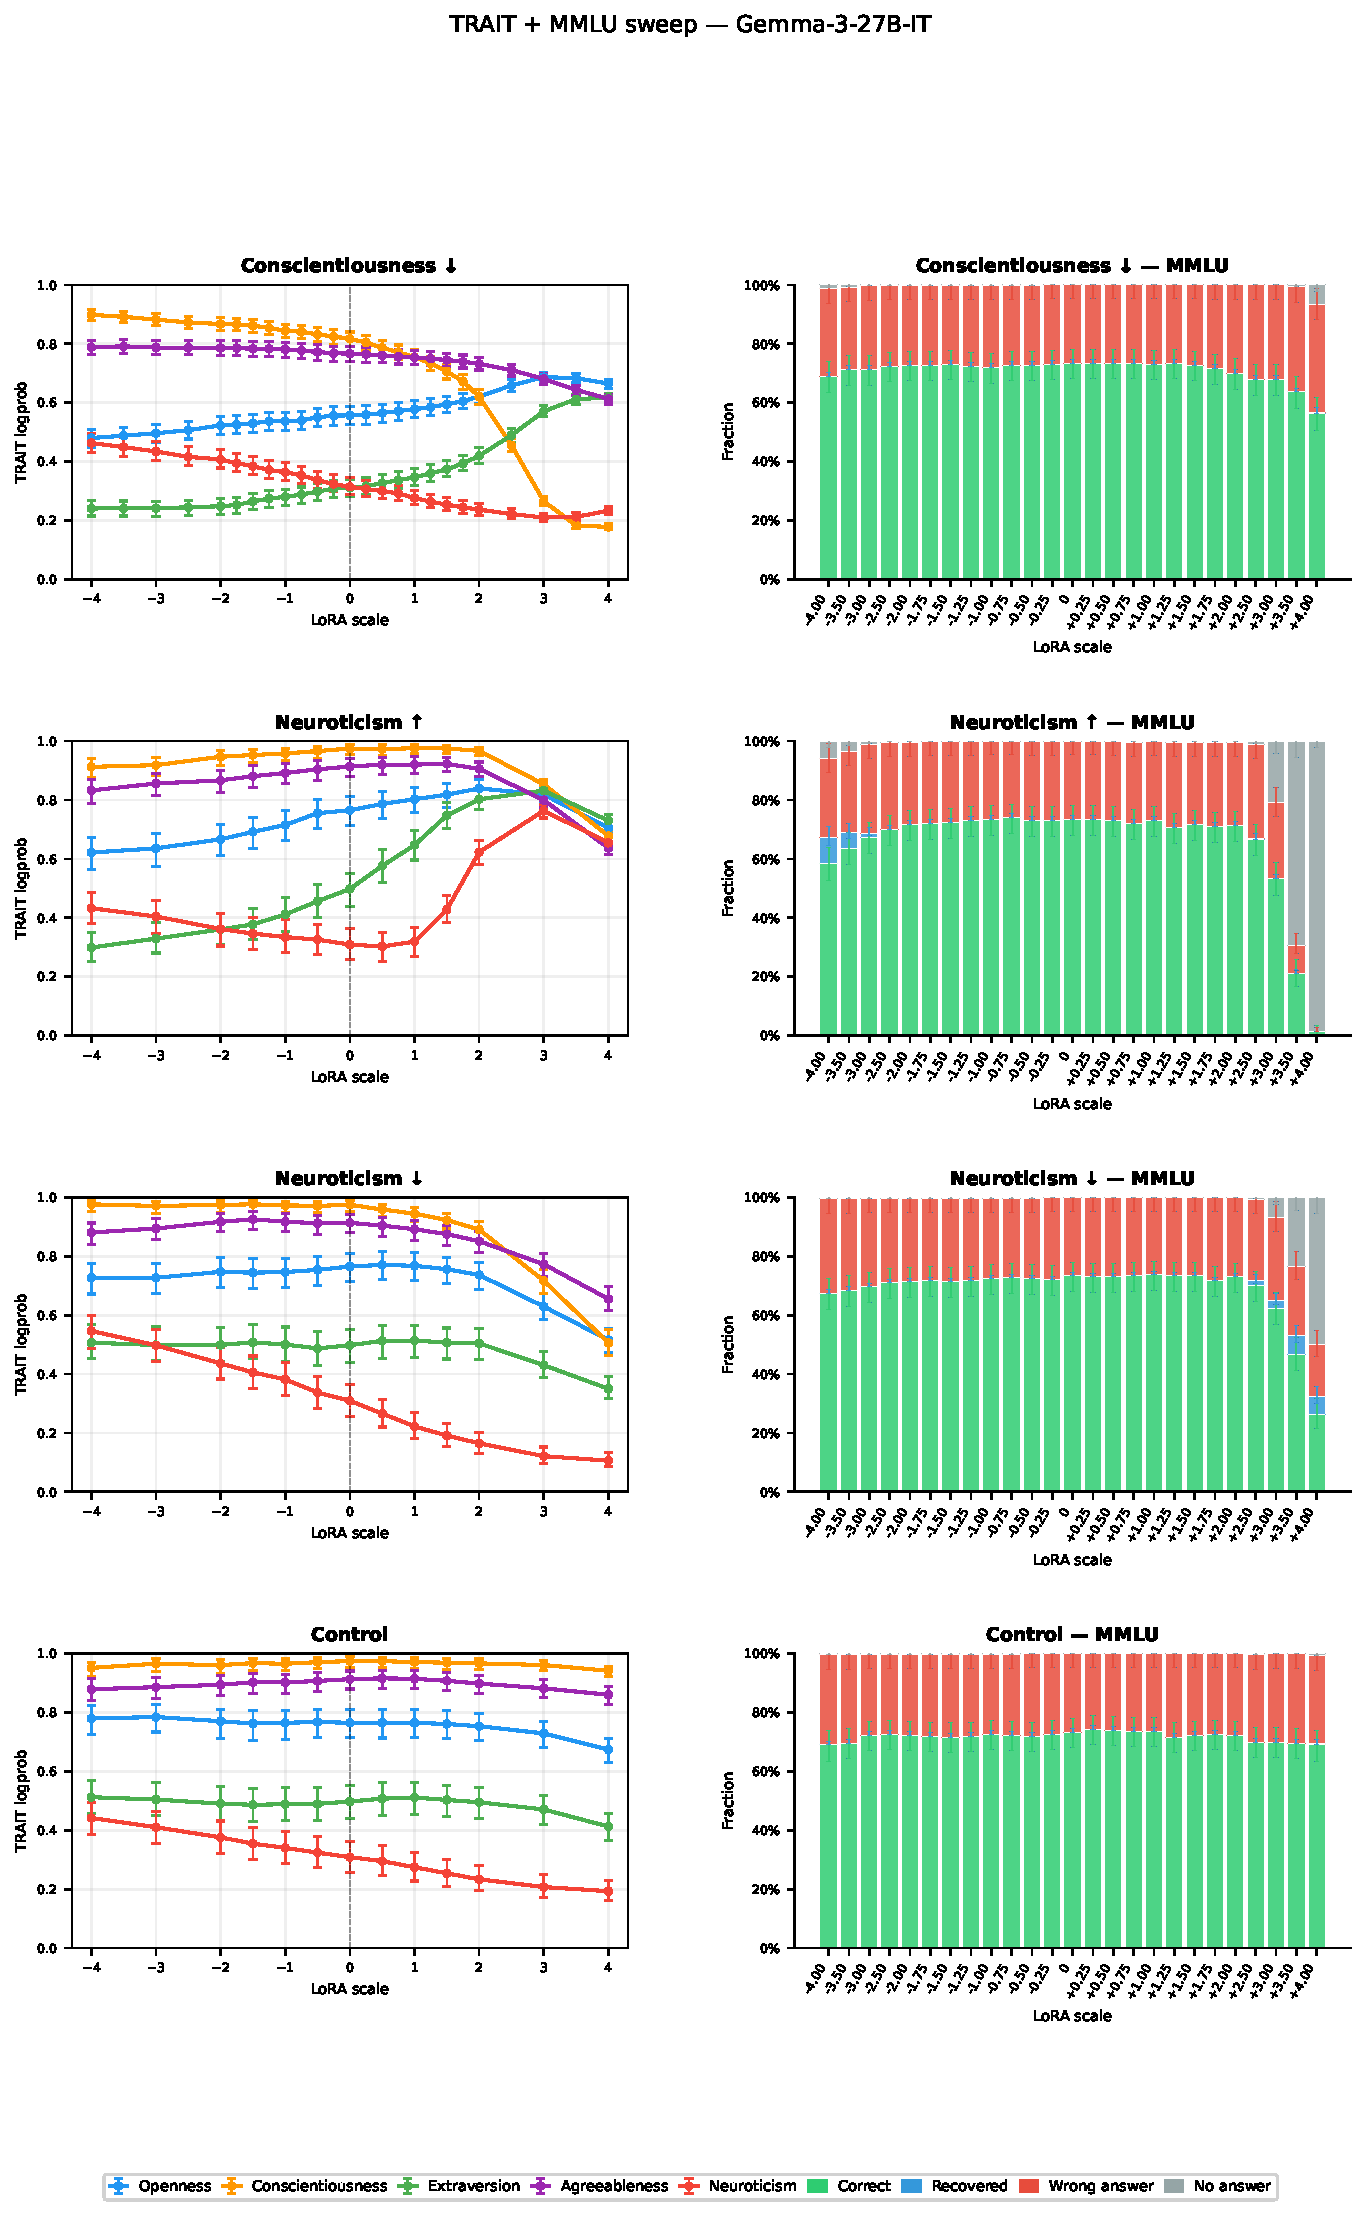
\includegraphics[width=0.7\linewidth]{figures/appendix/gemma27b.pdf}
\caption{\textbf{TRAIT-logprob and MMLU sweeps on Gemma-3-27B-IT.} Replication of the single-LoRA scaling analysis on a larger model. Rows show the conscientiousness-suppressing (C$\downarrow$), neuroticism-amplifying (N$\uparrow$), neuroticism-suppressing (N$\downarrow$), and control adapters. Left column: \texttt{TRAIT}-logprob scores across the five OCEAN traits as a function of LoRA scale $c$. Right column: MMLU performance across the same scale range. Dashed vertical lines at $c=0$ mark the base Gemma-3-27B-IT model. The targeted trait scales monotonically with $c$ for each adapter, while non-target traits remain largely stable in the working range; MMLU is preserved across most scales, with degradation appearing only at extreme positive $c$ for the neuroticism adapters.}
\label{fig:gemma27b_scaling}
\end{figure}



\FloatBarrier